% Source: graduate-coursework/Sp26/CSCE775/course_notes/bellman_equation_guide.tex
% Description: The Bellman Equation decomposes value into immediate and future components.

\documentclass[border=4pt]{standalone}
\usepackage{amsfonts}
\usepackage{amsmath}
\usepackage{amssymb}
\usepackage{amsthm}
\usepackage[T1]{fontenc}
\usepackage{graphicx}
\usepackage{tikz}
\usepackage{xcolor}
\usetikzlibrary{arrows.meta, positioning, shapes.geometric, calc, decorations.pathreplacing}

\definecolor{Garnet}{HTML}{73000a}
\definecolor{SecondaryBlue}{HTML}{466A9F}
\definecolor{SecondaryGreen}{HTML}{65780B}
\definecolor{FlatRed}{HTML}{CC2E40}
\definecolor{FlatDark}{HTML}{1F414D}
\definecolor{FlatYellow}{HTML}{CED318}
\definecolor{FlatGold}{HTML}{A49137}
\definecolor{LightGray}{HTML}{F0F0F0}

\renewcommand{\baselinestretch}{1.2}
\newcommand{\vocab}[1]{\textbf{\textcolor{Garnet}{#1}}}
\newcommand{\mathhighlight}[1]{\textcolor{SecondaryBlue}{#1}}

\begin{document}
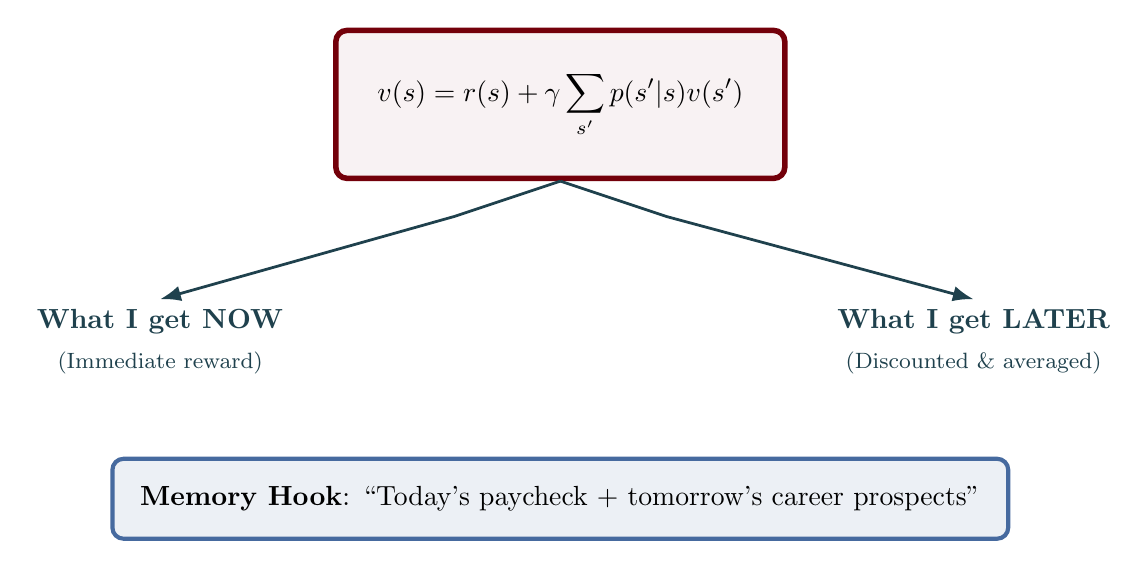
\begin{tikzpicture}[thick, scale=0.9]
        % Main equation box
        \node[draw=Garnet, line width=2pt, rounded corners, inner sep=15pt, fill=Garnet!5] (eq) at (0,0) {
            $v(s) = r(s) + \gamma \displaystyle\sum_{s'} p(s'|s) v(s')$
        };

        % Breakdown arrows
        \node[below left=1.5cm and 0.5cm of eq, align=center, text=FlatDark] (now) {
            \textbf{What I get NOW}\\
            \footnotesize (Immediate reward)
        };
        \node[below right=1.5cm and 0.5cm of eq, align=center, text=FlatDark] (later) {
            \textbf{What I get LATER}\\
            \footnotesize (Discounted \& averaged)
        };

        \draw[-{Latex}, FlatDark, line width=1pt] (eq.south) -- ++(-1.5,-0.5) -- (now.north);
        \draw[-{Latex}, FlatDark, line width=1pt] (eq.south) -- ++(1.5,-0.5) -- (later.north);

        % Memory hook
        \node[below=3.5cm of eq, draw=SecondaryBlue, line width=1.5pt, rounded corners, inner sep=10pt, fill=SecondaryBlue!10] {
            \textbf{Memory Hook}: ``Today's paycheck + tomorrow's career prospects''
        };
    \end{tikzpicture}
\end{document}
